\documentclass{article}

\usepackage{graphicx}

\title{Cloud Computing - Individual}
\author{Dave E. Craciunescu}
\date{2019.05.24}

\begin{document}

\maketitle

\section*{Módulo de Seguridad Azure}

Para la realización del análisis entre los diferentes módulos se hará la
comparativa entre las nubes de Azure y de Amazon Web Services.

Para la demostración del desarrollo e implementación de los servicios de la nube
de Azure se ha implementado y desarrollado el servicio de "Key Vault", descrito
por Azure mismo como "una manera de proteger las claves criptográficas y otros
secretos usados por las aplicaciones y los servicios en la nube".

La implementación de la misma en las máquinas virtuales que la quieran emplear
es extremadamente simple.

En primer lugar, ejecutaremos \textit{Azure Cloud Shell} para que la labor de
crear los diferentes recursos pueda ser mucho más simple y automatizable. La
interfaz visual online que proporciona Azure es altamente atractiva, pero esta
hace la labor de crear múltiples recursos muy tediosa y más un trabajo de
búsqueda y click de diferentes opciones en los que se pierde el hilo del
desarrollo entre acción y acción.

\begin{figure}[h!]
    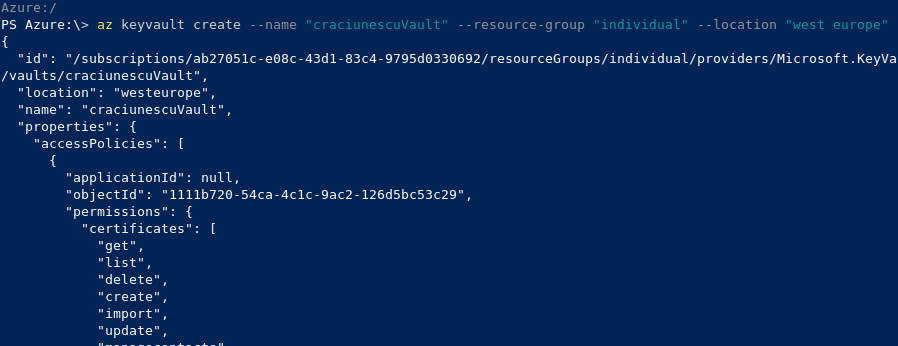
\includegraphics[width=\linewidth]{./Selection_011.png}
    \caption{Creación de un Vault}
\end{figure}

Una vez tengamos el recurso creado, podremos emplear el \textit{KeyVault} dentro
de los diferentes recursos que nos ofrezca Azure mismo. Un ejemplo claro sería
el de guardar diferentes credenciales dentro del Vault desde máquinas virtuales
creadas en Azure. Esto se puede conseguir de la siguiente manera:

\begin{figure}[h!]
    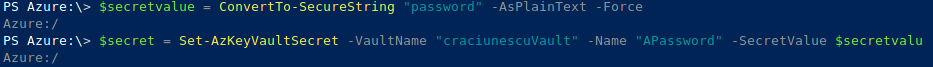
\includegraphics[width=\linewidth]{./Selection_012.png}
    \caption{Creación de un Secreto}
\end{figure}

Con esto ahora somos capaces de guardar diferentes "secretos", según Azure los
llama y conseguirlos sin tener que preocuparnos por más que acordarnos bajo qué
nombre los guardamos.

Si ahora quisiésemos recuperar la clave asociada a "APassword" no tendríamos que
hacer nada más que lo siguiente.

\begin{figure}[h!]
    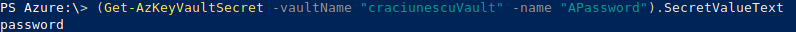
\includegraphics[width=\linewidth]{./Selection_013.png}
    \caption{Obtener Secreto}
\end{figure}

Este tipo de acciones se pueden \textit{nestear} dentro de nuestros programas
para que el uso de información privilegiada o secretos se vea extremadamente
simplificado y la labor de tener que tener apuntadas contraseñas o memorizar
claves alfanuméricas complicadas desaparezca.

\section*{Análisis Módulo de Seguridad de Azure}

En esta sección se podrá encontrar un análisis de los productos de seguridad más
importantes de la nube de Microsoft Azure. Algunos de ellos no han
sido incluidos debida su generalidad y conocimiento común de los mismos. 

\subsection*{Azure Sentinel}

La herramienta de \textit{Azure Sentinel} se puede describir como una
\textit{'plataforma de administración de eventos e información de seguridad
nativa en la nube que utiliza inteligencia artificial integrada para facilitar
el análisis rápido de grandes volúmenes de datos en una empresa'}. 

La herramienta de \textit{Azure Sentinel} es una herramienta automatizada de seguridad dentro
de la empresa caracterizada por los siguientes elementos:

(1) Recopilación de datos de toda la infraestructura tanto en el entorno local
como en las diversas nubes. Lo que consigue Sentinel es conglomerar todos los
datos que sea capaz de agregar de cualquier entorno o fuente y conseguir
conclusiones a partir de millones de registros en apenas segundos. 

(2) Además, gracias al uso de la inteligencia artificial y a la
gran experiencia de Microsoft dentro del mundo de la ciberseguridad, Sentinel es
capaz de detectar amenazas no descubiertas con anterioridad e incluso minimizar
la cantidad de falsos positivos, lo que era un problema en el pasado.

(3) Como ya se ha mencionado, Sentinel no solo emplea la Inteligencia Artificial
para Investigación de las diferentes amenazas con herramientas de Inteligencia
Artificial y búsqueda de actividad sospechosa a escala.

(4) Respuesta a los incidentes con rapidez orquestando y automatizando las
tareas comunes integradas.

Es importante mencionar que el servicio que ofrece Azure Sentinel se integra
perfectamente con el resto de herramientas de la suite de Microsoft Azure y las
herramientas de Office 365, lo que proporciona un alto nivel de funcionalidad a
la hora de usar el servicio para la empresa. Desde un punto de vista
funcional, la mayoría de empleados/usuarios no sabrán usar más de un par de
teconologías, así que no tener que forzar a que se adapten a una nueva al
contratar el servicio es un gran punto a favor.

\subsection*{Azure Security Center}

El servicio de Azure Security Center junta muchos recursos de seguridad de Azure
y los agrupa en un \textit{centro de seguridad} como tal. El funcionamiento de
este centro de seguridad es relativamente simple y ataca desde 4 flancos
principales.

\subsubsection*{Protección para servidores Linux y Windows}
El centro de seguridad ayuda a salvaguardar los servidores y los clientes
Windows con el \textit{Windows Defender Advanced Threat Protection} y ayuda a
los servidores Linux con analíticas de comportamiento. Para cada ataque o
intento de ataque sobre los servidores, Security Center creará notificaciones
detalladas con información relevante sobre el evento.

\subsubsection*{Protección para aplicaciones nativas a la nube}
Este se puede centrar en las aplicaciones nativas a la nube como páginas o
plug-ins expuestos que son frecuentemente atacados. El centro de seguridad crea
diferentes reglas para el firewall que cambian automáticamente para actualizarse
con los diferentes ataques que se vayan registrando e incrementar la seguridad
de las aplicaciones con el tiempo.

\subsubsection*{Protección para los datos}
Gracias a las labores de los expertos en big data y machine learning, Security
Center es capaz de reconocer estados o \textit{queries} poco seguras o anómalas,
ataques de inyección de SQL y cualquier otro tipo de ataque que pueda centrarse
en las bases de datos de Azure. También existe un sistema de notificaciones en
tiempo real que hace al administrador saber inmediatamente si cualquier tipo de
vulnerabilidad de este estilo ha sido encontrada. Entre otras características
que pueden proteger los datos se encuentran los accesos desde rutas poco comunes
o conexiones anónimas poco comunes.

\subsection*{Key Vault}

El servicio de administración de claves de Microsoft Azure es una herramienta
muy famosa empleada para facilitar cualquier acción relacionada con el
almacenamiento de claves o información privilegiada de cualquier tipo. Según
Azure mismo, \textit{Key Vault} se puede usar para cifrar claves y pequeños
secretos, como contraseñas que usan claves almacenadas en módulos de seguridad
hardware. El funcionamiento de la herramienta ya ha sido explicado en la parte
específica, por tanto no se reiterará. De cualquier manera, se recomienda el uso
de esta herramienta a cualquier empresa que tenga en cuenta la seguridad de sus
claves.

\subsection*{Azure Active Directory}
Azure Active Directory es un servicio de administración de acceso y de
identidades basado en la nube de Microsoft que ayuda a los recursos de acceso y
de inicio de sesión de los empleados en: recursos externos, como Microsoft
Office 365, y recursos internos, como aplicaciones de la red corporativa y la
intranet.

Algunas de las características más importantes que vienen con Azure Active
Directory son las siguientes:

\subsubsection*{Acceso seguro a aplicaciones}
Gracias a Azure Active Directory los usuarios podrán conectarse a sus
aplicaciones y datos sin problema. El sistema es capaz de integrar rápidamente
los diferentes niveles de autenticación de distintas aplicaciones y centralizar
el acceso a las mismas en una única plataforma que compruebe la identidad.
Gracias a la herramienta desaparecen los días en los que hay que escribir una
contraseña diferente para acceder a cada servicio.

\subsubsection*{Protección integral de la identidad}
Gracias a diferentes características internas de AAD, como el aprendizaje
automático, la herramienta en cuestión es capaz de captar patrones en la manera
de autenticación de los diferentes usuarios e intentar analizar diferentes
señales para descifrar con más factores si el usuario es quien dice ser. Existe
la posibilidad de que alguien conozca la contraseña de un usuario en concreto y
quiera acceder a su cuenta furtivamente, AAD está trabajando activamente para
que el nivel de reconocimiento no pare solo en la introducción de la contraseña,
sino también se puedan analizar patrones a la hora de hacerlo que ayuden a la
hora de identificar al usuario.

\subsubsection*{Gran abanico de aplicaciones compatibles}
Gracias a la gran funcionalidad de todos los servicios de Microsoft,
\textit{Microsoft Active Directory} es empleado por una serie masiva de
plataformas de peso, entre las cuales se encuentran nombres como: salesforce,
SAP Concur, workplace, Blackboard, myday, canvas, y muchas otras. 

Esto debería ser suficiente para demostrar que Active Directory funciona y vale
la pena como servicio para una empresa. 

\subsection*{Azure DDoS Protection}
Los ataques por denegación de servicio distribuido son uno de los problemas de
seguridad y disponibilidad más extendidos a los que se enfrentan los clientes
que mueven sus aplicaciones a la nube. Un ataque DDoS intenga agotar los
recursos de una aplicación haciendo que esta no esté disponible para los
usuarios legítimos. Los ataque DDoS pueden ir dirigidos a cualquier punto de
conexión que sea públicamente accesible a través de internet.

Esta herramienta es capaz de proporcionar un abanico de características muy
útiles para la empresa, entre las que se pueden encontrar las siguiente:

\subsubsection*{Supervisión continua del tráfico}
Se pueden crear unas reglas de protección o unos "límites" en la supervisión del
tráfico. Azure DDoS Protectión analizará constantemente y de forma
ininterrumpida si estos límites se sobrepasan, y solo actúa en el momento en el
que se haya roto la barrera para mitigar el posible ataque DDoS.
    
\subsubsection*{Protección llave en mano}
Gracias a la configuración simplificada del servicio y la gran integración con
el resto de herramientas de la suite de Microsoft, se puede proteger de
inmediato todos los recursos de una red virtual privada desde el momento en el
que se habilita la protección misma. La intervención del usuario no es necesaria
en ningún momento, a no ser que se quieran cambiar las políticas de limitación
de tráfico. El servicio se podría añadir a la red que queramos analizar, no
volver a tocar, y este funcionar perfectamente sin ningún tipo de intervención
humana.

\subsubsection*{Análisis de Ataque}
La protección es importante, pero saber quién ha atacado también puede ayudar de
cara al futuro, con esto en mente, Azure DDoS Protection fabrica informes
detallados en tiempo real sobre el ataque y un resumen completo del mismo una
vez este acabe. Esta documentación puede significar mucho a la hora de hacer
análisis de riesgos o tener que pasar pruebas de certificaciones, auditorías
legales, etc.\

\subsubsection*{Servicio de Alerta de Ataques}
Como el lector ávido puede haber deducido, ya que el analizador de ataques es
capaz de mostrar información casi en tiempo real, de la misma manera el sistema
es capaz de \textit{advertir} de que este está sufriendo un ataque. Estas,
además, se pueden configurar y conectar con otros elementos de la red de
herramientas de Azure y notificar al adminsitrador por correo electrónico,
portal de Azure, etc.\

\end{document}
